\section{K-means Algorithm}\label{sec:kmeans}

The first method considered for automating the measurement process is the K-means algorithm.
K-means \cite{lloyd1982least} is a clustering technique used in unsupervised machine learning. It works by minimizing a function that measures the quality of clusters. The algorithm starts by randomly selecting $k$ points from the dataset as cluster centers. Each data point is then assigned to the nearest center based on distance. The centers are updated by calculating the geometric mean of the points in each cluster, and this process repeats until convergence.

K-means is useful for separating image regions based on color similarity, which matches the goal of image segmentation in this work. One of its main advantages is that it does not require pre-existing labels, which makes it a good starting point when labels are unavailable.

However, the algorithm has several limitations. Since it relies mainly on color, it struggles with images where regions have similar colors. For example, in the third image in Figure~\ref{fig:three-images}, oxidation appears under or over the coating layer, making it difficult to segment. Also, the same K-means settings cannot be used for all coatings, as shown in Figure~\ref{fig:three-images}; different coatings have different numbers of layers and colors.

The value of $k$ needs to be manually set for each image set, and additional post-processing is often required to isolate the desired cluster. As shown in Figure~\ref{fig:kmean}, K-means often fails to separate oxidation from the coating layer due to their similar pixel values, and it frequently clusters them together.

\begin{figure} [H]
    \centering 
    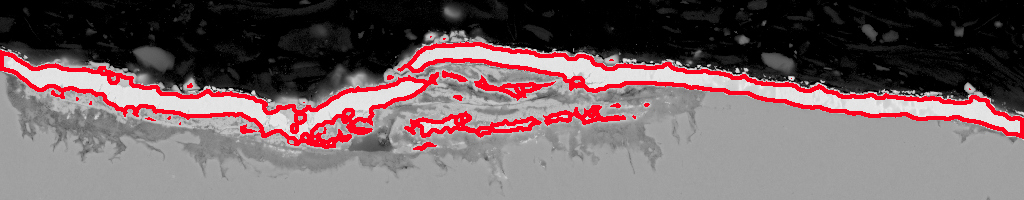
\includegraphics[width=0.8\linewidth]{PICTURES/kmeans/04.png} 
    \caption{Highlighted coating layers predicted using K-means.} 
    \label{fig:kmean} 
\end{figure}